\documentclass[10pt]{article}
\usepackage{icmlko}

\icmlmeta{IP 파운데이션 월드모델}{305}{판정 셋 중 어느 것도 뺄 근거가 아니다}{어제 만든 겹침 도구의 남은 판정 하나를 시험했다 --- ① 보다 자리당 1.57배 비싸다}

\begin{document}

\twocolumn[
\icmlheader

\begin{abstract}
노트 301이 검사 ①(``안 오른다'')로 축을 빼면 판이 갈릴 만큼 나빠진다는 것을
보이고 \textbf{``검사 ③ 은 그대로 둔다''}고 적었다. \textbf{그 문장을 안
쟀다.} 어제 \texttt{lab/overlap.py} 를 만들어 모든 실행의
\texttt{cfg["겹침"]} 에 붙였으므로, 그 판정 셋 중 몇이 제거를 정당화할 수
있는지는 \textbf{도구 자체의 문제}다. 재기 전에 예측을 적고
(\texttt{preregister\_maskdup.json}) ``이미 있다'' 17자리를 껐다. 결과 ---
판 0.4851 $\to$ \textbf{0.4782}, $\Delta{=}{-}0.0068$, 짝SE 0.0035,
$t{=}{-}1.96$, 문턱 0.0070. \textbf{못 가른다} --- 0.0002 차이로.
그런데 \textbf{자리당으로 보면 ③ 이 ① 보다 비싸다}: ① 47자리가 자리당
$-2.57{\times}10^{-4}$, ③ 17자리가 \textbf{$-4.00{\times}10^{-4}$},
\textbf{1.57배}다. 예측(``$-$0.004 $\sim$ $-$0.010, 47자리보다 작게'')은
크기로는 맞고 방향 해석으로는 틀렸다 --- 총량이 작은 것은 자리 수가 적어서지
자리가 싸서가 아니다. \textbf{그래서 겹침 도구의 세 판정 중 어느 것도
축을 뺄 근거가 못 된다.} 덤으로 \textbf{도서는 자기 축을 하나도 안 껐는데
$-$0.0407($t{=}{-}2.12$)로 제일 크게 움직인다} --- 남의 도메인 축을 끄면
공유 적합이 바뀌고, 노트 303이 잰 대로 도서가 제일 많이 빌리는 도메인이다.
\end{abstract}
]

\section{안 잰 문장이 있었다}

노트 301의 마지막 절이 이렇게 끝난다.

\begin{center}\small
``\textbf{① 을 이유로 축을 빼면 안 된다}가 이 노트의 결론이고,\\
③ 은 그대로 둔다.''
\end{center}

그 문장에 근거가 없었다. 그리고 논리적으로 ③ 도 같은 맹점을 가진다 ---
\textbf{③ 은 \emph{그 도메인 안에서} 공유 축을 통제하고 남는지를 묻지,
그 값이 \emph{남의 도메인에서 배운 함수}에 들어가서 하는 일을 묻지 않는다.}
노트 301이 보인 경로가 바로 그것이다.

\begin{center}\footnotesize
\begin{tabular}{ll}
\hline
판정 & 뜻 \\
\hline
새롭다 36 & ① ③ 둘 다 통과 \\
\textbf{이미 있다} 17 & ① 통과 · ③ 탈락 \\
안 오른다 47 & ① 탈락 --- \textbf{노트 301이 시험함} \\
\hline
\end{tabular}
\end{center}

\section{못 가른다. 그런데 자리당은 더 비싸다}

\begin{figure*}[t]
\centering
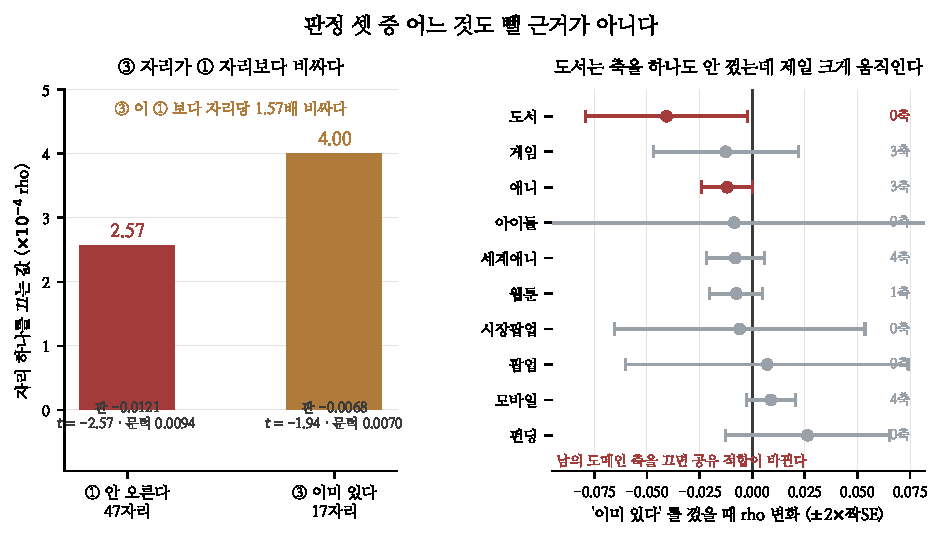
\includegraphics[width=\textwidth]{figs/neither.pdf}
\caption{왼쪽 --- 자리 하나를 끄는 값. 오른쪽 --- ``이미 있다'' 를 껐을 때
도메인 $\rho$ 의 변화($\pm$2$\times$짝SE, 부트스트랩 400).}
\end{figure*}

\begin{center}\small
\begin{tabular}{lrr}
\hline
& ① 안 오른다 & ③ 이미 있다 \\
\hline
자리 & 47 & 17 \\
판 $\Delta$ & $-$0.0121 & $-$0.0068 \\
짝SE & 0.0047 & 0.0035 \\
$t$ & \textbf{$-$2.58} & $-$1.96 \\
문턱 & 0.0094 & 0.0070 \\
판정 & \textbf{갈린다} & 못 가른다 \\
\hline
\textbf{자리당} ($\times10^{-4}$) & $-$2.57 & \textbf{$-$4.00} \\
\hline
\end{tabular}
\end{center}

\textbf{총량은 ① 이 크고 자리당은 ③ 이 크다.} ③ 자리가 ① 자리보다
\textbf{1.57배} 비싸다 --- 당연하다면 당연하다. ``이미 있다''는 검사 ① 을
\emph{통과한} 축이므로 제 도메인에서도 라벨과 관계가 있다.

\paragraph{예측을 어떻게 틀렸나} 미리 적은 것: ``무너진다 --- 다만 47자리보다
작게. 판 $\Delta$ $-$0.004 $\sim$ $-$0.010.'' 점추정 $-$0.0068 은 그 안에
들어왔지만 \textbf{``47자리보다 작게''를 ``자리가 싸다''로 읽었던 것이
틀렸다.} 자리 수를 안 나누고 총량만 비교하려던 셈이다. 사전 등록에
``자리당으로 견준다''를 적어 둔 것이 이번에는 살렸다.

\section{축을 하나도 안 껐는데 움직인다}

\begin{center}\footnotesize
\begin{tabular}{lrrrr}
\hline
도메인 & $\Delta$ & 짝SE & $t$ & 끈 축 \\
\hline
\textbf{도서} & \textbf{$-$0.0407} & 0.0192 & \textbf{$-$2.12} & \textbf{0} \\
게임 & $-$0.0126 & 0.0172 & $-$0.73 & 3 \\
애니 & $-$0.0119 & 0.0061 & $-$1.94 & 3 \\
아이돌 & $-$0.0085 & 0.0553 & $-$0.15 & 0 \\
세계애니 & $-$0.0080 & 0.0069 & $-$1.16 & 4 \\
웹툰 & $-$0.0075 & 0.0063 & $-$1.20 & 1 \\
시장팝업 & $-$0.0060 & 0.0298 & $-$0.20 & 0 \\
팝업 & $+$0.0072 & 0.0336 & $+$0.21 & 0 \\
모바일 & $+$0.0089 & 0.0058 & $+$1.53 & 4 \\
펀딩 & $+$0.0263 & 0.0195 & $+$1.35 & 0 \\
\hline
\end{tabular}
\end{center}

\textbf{도서는 ``이미 있다'' 자리가 하나도 없다.} 그런데 제일 크게
움직인다($-$0.0407, $t{=}{-}2.12$). \textbf{남의 도메인 축을 끄면 공유 적합이
바뀌고 도서가 그 변화를 제일 크게 받는다} --- 노트 303이 도서를 판에서 제일
많이 빌리는 도메인(제 점수의 35\%)으로 쟀는데, 그 도메인이 남의 축 변화에도
제일 민감하다. \textbf{같은 성질의 두 얼굴이다.}

가드 열아홉 통과.

\section{그래서 도구의 쓸모를 다시 적는다}

\begin{center}\footnotesize
\begin{tabular}{lll}
\hline
판정 & 뺄 근거인가 & 무엇에 쓰나 \\
\hline
안 오른다 47 & \textbf{아니다}(노트 301) & 빌리는 자리 찾기 \\
이미 있다 17 & \textbf{아니다}(이 노트) & 자료 수집 우선순위 \\
새롭다 36 & --- & 안 뺀다 \\
\hline
\end{tabular}
\end{center}

\textbf{겹침은 제거의 근거가 아니라 지도다.} ``안 오른다''가 몰린 도메인
(도서 9 · 펀딩 9)이 노트 303에서 제일 많이 빌리는 도메인으로 나왔다 ---
같은 표가 \emph{빼야 할 곳}이 아니라 \emph{빌리고 있는 곳}을 가리키고
있었다. 그리고 ``이미 있다''는 \textbf{같은 정보를 두 경로로 받고 있다}는
뜻이므로 \emph{새 자료를 모을 때 거기를 피하라}는 신호다.

\paragraph{남은 것}
\begin{center}\small
\begin{tabular}{ll}
\hline
갈래 & 왜 \\
\hline
``새롭다'' 36 도 & 셋째 대조 --- 제일 비쌀 듯 \\
겹침 표를 지도로 & 이름을 ``뺄 것''에서 바꾼다 \\
도서에 축을 더 & 빌리는 도메인이 받을 자리 \\
피처 위약 & 노트 302의 갈래 --- 돌고 있다 \\
\hline
\end{tabular}
\end{center}

\paragraph{규약} \textbf{도구를 만들면 그 도구의 판정마다 시험을 붙여라.}
어제 겹침 도구를 만들면서 판정을 셋으로 냈는데, 이틀에 걸쳐 둘을 시험하니
\textbf{둘 다 제거를 정당화 못 한다.} 도구가 내는 이름이 곧 다음 수를
정하므로(노트 301에서 ``잡음''이라는 낱말 하나가 판을 0.0121 떨어뜨렸다)
\textbf{이름을 붙이는 것과 그 이름으로 무엇을 할지는 따로 재야 한다.}
그리고 \textbf{총량으로 견주지 말고 단위로 견주어라} --- 이번 예측이
틀린 자리가 정확히 거기다.

\end{document}
